\section{Administrative Area}
The Administrative Area is the AllSpark's section interested on the management of its lifecyle. All the purposes to achieve here contribute to the Company management, and the implicit work has the primary objective of mantaining the operativity. It's important to employees direct related to these functions bearing in mind the position of the Company with respect the relations with the specific business sector.

The group of employee related in this Area are grouped in the ``Administrative'' organization nit according with the Working Structure in figure \ref{2img:working}. All processes are supervised by the Chief Executive Officer (CEO) who monitors the business process according with his conceptual ideas and his primary role of AllSpark's leader.

\subsection{Billing}
This process provides support for the definition of the appropriate remuneration for the service supplied.
The process takes into account the history of project development and the details defined in the contract, in order to check if they match or if some extra features have been during the development phase. The employees mainly involved are Business Consultant, Secretary and the CEO.

Image \ref{2img:billing} shows how this process is realized in practice, focusing on the resources used and the targets for each activity. The goal of this process is to provide a fair billing to the customer, balanced on the services actually delivered.\\

\begin{figure}[ht!]
\begin{centering}
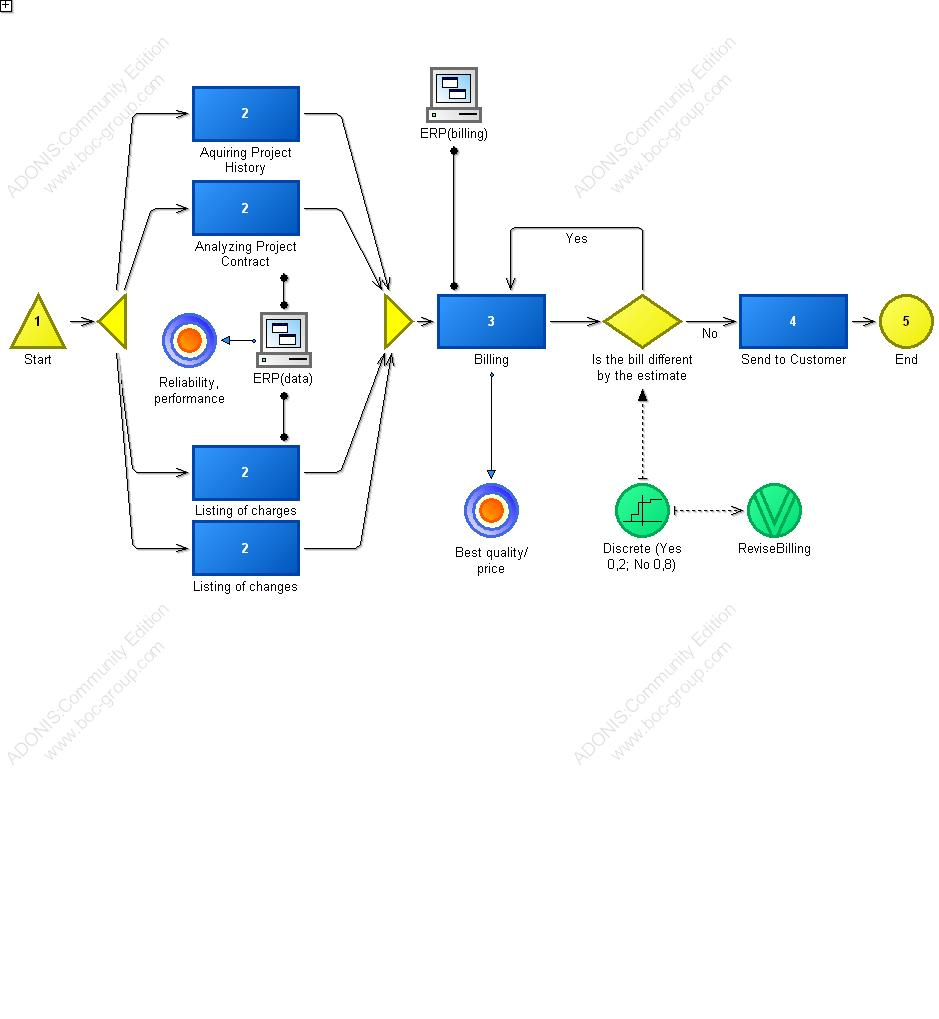
\includegraphics[scale=0.45, angle=90]{assign2/adonis/imgs/billing.jpg}
\caption{AllSpark billing process.}
\label{2img:billing}
\end{centering}
\end{figure}


\subsubsection{Path Analysis}
The analysis of possible paths results five correspondence, one with the 80,40\% of probability to be performed. For simulation's convention the number of these processes per month is configured on three element on average. The result obtained coincide with the expectations.

\begin{alltt}
Probability:   80,4000\%
Execution time:  00:000:00:24:20
Waiting time:  00:000:00:05:00
Resting time:  00:000:00:11:10
Transport time:  00:000:00:01:00
Cycle time:  00:000:00:29:20
Costs:  27,100000

Billing 0.3 (Business process model)

========================================
Process start: Start
Parallelity: Parallelity-25245
    *
    Activity: Aquiring Project History
    *
    Activity: Analyzing Project Contract
    *
    Activity: Listing of charges
    *
    Activity: Listing of changes
Merging: Merging-25248
Activity: Billing
Decision: Is the bill different by the estimate --> ReviseBilling = 'No'
Activity: Send to Customer
End: End
\end{alltt}


\subsubsection{Capacity Analysis}
The capacity analysis of the process illustrates the specified timing and costs forseen for the single activities. Morevover it exlicities the Performer associated to each activity in order to check the responsibility for each step of the Business Process. The Cycle time is as expected greater than the Execution time due to some calculus correction or, with more probability, unforseen intervent or additional features that appears during the project life.

\begin{table}
\centering
{\tiny
\begin{tabular}{|l|l|l|l|l|l|l|}
Business process&Activity&Performer&Number&Execution time&Cycle time&Costs\\
\hline
Billing 0.3&&&&00:000:00:24:51&00:000:00:32:42&33,575000\\
\hline
&Aquiring Project History &&1,000000&00:000:00:10:00&&1,300000\\
\hline
&&Secretary&1,000000&00:000:00:10:00&&1,300000\\
\hline
&Analyzing Project Contract &&1,000000&00:000:00:10:00&&0,200000\\
\hline
&&Secretary&1,000000&00:000:00:10:00&&0,200000\\
\hline
&Listing of charges &&1,000000&00:000:00:01:00&&0,300000\\
\hline
&&Business consultant&1,000000&00:000:00:01:00&&0,300000\\
\hline
&Billing &&1,259000&00:000:00:02:31&&31,475000\\
\hline
&&Business consultant&1,259000&00:000:00:02:31&&31,475000\\
\hline
&Listing of changes &&1,000000&00:000:00:01:00&&0,200000\\
\hline
&&Secretary&1,000000&00:000:00:01:00&&0,200000\\
\hline
&Send to Customer &&1,000000&00:000:00:00:20&&0,100000\\
\hline
&&Secretary&1,000000&00:000:00:00:20&&0,100000\\
\hline
Total&&&&00:000:00:24:51&&33,575000
\end{tabular}
}
\caption{Capacity analysis for Billing.}
\end{table}
%

%

\subsection{Bureaucracy Management}
The "Bureaucracy Management" business process aims to regulate the set of codes from which AllSpark depends on. The scope of this sequence is monitoring the country laws and the licences estabilished, check the efficiency of the responsibility charge and undertake the needed changes to restore the legality.

Since the task is actual demanding the roles it has associated are all fitting the "Administrative" organizational unit according to the Working structure in \ref{2img:working}. Particular the secretary is directed the mainly connect to all of the activities as described in the above structure.

The figure \ref{2img:bureaucracy} shows the graphical representation, focusing on the management side of the topic than the pratical step.\\

\begin{figure}[ht!]
\begin{centering}
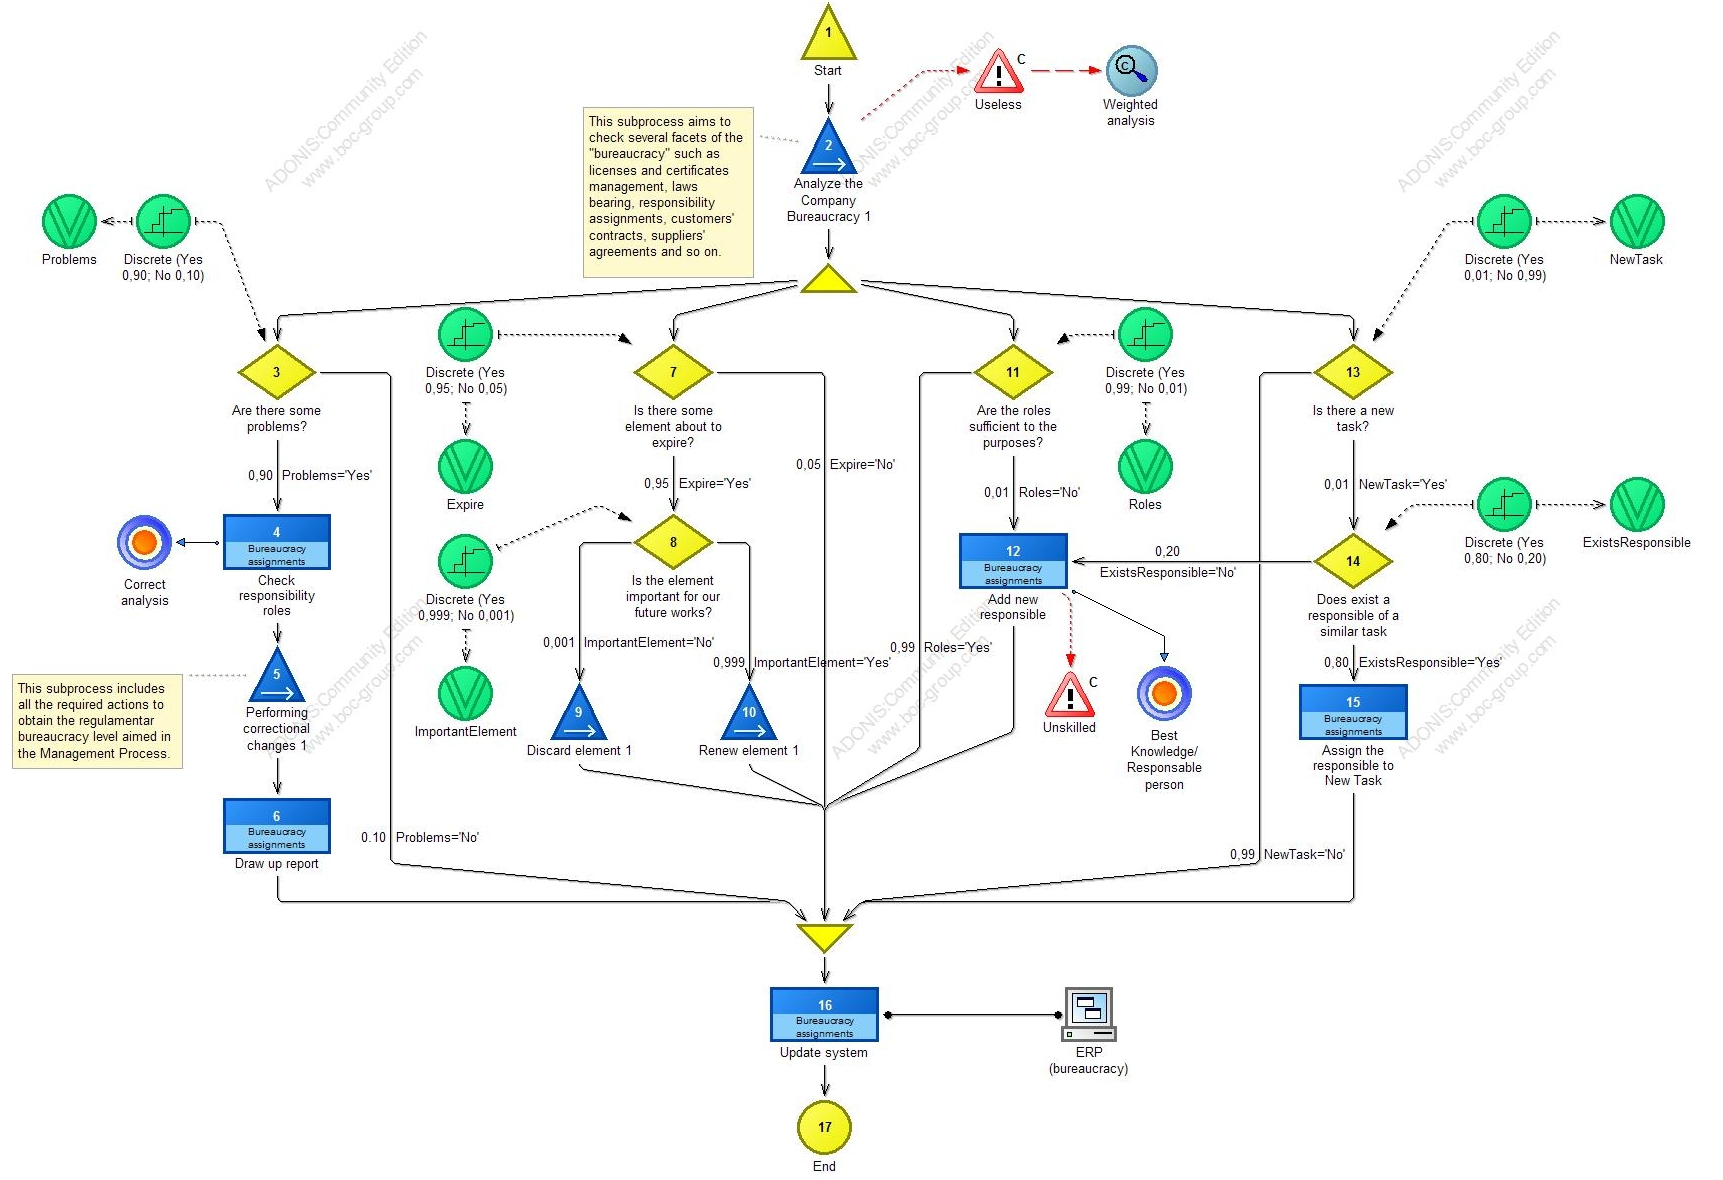
\includegraphics[scale=0.30, angle=90]{assign2/adonis/imgs/bureaucracy.jpg}
\caption{AllSpark bureaucracy management.}
\label{2img:bureaucracy}
\end{centering}
\end{figure}


\subsubsection{Path Analysis}
Ten paths were discovered by the analysis of the modelization; the first leads with the 84,70\% probability to be performed. This result is coherent with the foreseen one since perform the ``usual'' way modeled to accomplish the task. This process is performed with minor frequency than others and so it indicates a stable company assessments that involve in updating since AllSpark aims to mantain the same structure.

\begin{alltt}
Probability:   84,7000\%
Execution time:  00:000:01:55:00
Waiting time:  00:000:00:11:00
Resting time:  00:000:00:16:00
Transport time:  00:000:00:15:00
Cycle time:  00:000:01:55:00
Costs:  2030,850000

Bureaucracy Management 0.1 (Business process model)
========================================
Process start: Start
Subprocess: Analyze the Company Bureaucracy
Parallelity: Parallelity-37827
    *
    Decision: Are the roles sufficient to the purposes? --> Roles='Yes'
    *
    Decision: Is there a new task? --> NewTask='No'
    *
    Decision: Are there some problems? --> Problems='Yes'
    Activity: Check responsibility roles
    Subprocess: Performing correctional changes
    Activity: Draw up report
    *
    Decision: Is there some element about to expire? --> Expire='Yes'
    Decision: Is the element important for our future works? --> ImportantElement='Yes'
    Subprocess: Renew element
Merging: Merging-37855
Activity: Update system
End: End

Bureaucracy Management 0.1 (Business process model) --> Analyze the Company Bureaucracy 1 (Business process model)
========================================
Process start: Start
Activity: Analyze the Company Bureaucracy
End: End

Bureaucracy Management 0.1 (Business process model) --> Renew element 1 (Business process model)
========================================
Process start: Start
Activity: Renew element
End: End

Bureaucracy Management 0.1 (Business process model) --> Performing correctional changes 1 (Business process model)
========================================
Process start: Start
Activity: Performing correction
End: End
\end{alltt}


\subsubsection{Capacity Analysis}
In the capacity analysis of the process reported below, is possible to observe that the task is very wasting both in terms of time and in costs.

It is important to underline that the Process is defined to be performed at least once a month and the result obtained by the simulation agree in the forseen time employed, this is defined by a higher probability of the choice in the modeled Business Process.

\begin{landscape}
\centering
\begin{table}
{\tiny
\begin{tabular}{|l|l|l|l|l|l|l|}
Business process&Activity&Performer&Number&Execution time&Cycle time&Costs\\
\hline
Bureaucracy Management 0.2&&&&00:000:01:46:01&00:000:01:49:03&1919,760040\\
\hline
&Check responsibility roles&&0,899000&00:000:00:26:58&&26,970000\\
\hline
&&Secretary&0,899000&00:000:00:26:58&&26,970000\\
\hline
&Add new responsible&&0,010000&00:000:00:00:09&&0,000500\\
\hline
&&Secretary&0,010000&00:000:00:00:09&&0,000500\\
\hline
&Update system&&1,000000&00:000:00:05:00&&0,050000\\
\hline
&&Secretary&1,000000&00:000:00:05:00&&0,050000\\
\hline
&Draw up report&&0,899000&00:000:00:17:59&&0,179800\\
\hline
&&Secretary&0,899000&00:000:00:17:59&&0,179800\\
\hline
&Assign the responsible to New Task&&0,009000&00:000:00:00:01&&0,000090\\
\hline
&&Secretary&0,009000&00:000:00:00:01&&0,000090\\
\hline
&Analyze the Company Bureaucracy&&1,000000&00:000:00:10:00&&0,200000\\
\hline
&&Secretary&1,000000&00:000:00:10:00&&0,200000\\
\hline
&Performing correction&&0,899000&00:000:00:26:58&&0,359600\\
\hline
&&Secretary&0,899000&00:000:00:26:58&&0,359600\\
\hline
&Renew element&&0,946000&00:000:00:18:55&&1892,000000\\
\hline
&&Secretary&0,946000&00:000:00:18:55&&1892,000000\\
\hline
&Discard element&&0,001000&00:000:00:00:00&&0,000050\\
\hline
&&Secretary&0,001000&00:000:00:00:00&&0,000050\\
\hline
Total&&&&00:000:01:46:01&&1919,760040
\end{tabular}
}
\caption{Capacity analysis for Bureaucracy Management.}
\end{table}
\end{landscape}
%

%

\subsection{Financial support}
The "Financial support" business process wokrs on the management of the Company's financial status with monitoring the growing opportunities as primary target, but not least also to check the AllSpark's trend in order to mantain the position gained. Reliability is a important objecttive to reach in this process since a wrong planning may have serious reflections in the future of the Company (and, of course, of its employees).

The primary responsible of all the business process is the business consultant who is assisted by the secretary and supervised for decision by the CEO.

The figure \ref{2img:financial_sup} reports the representation of the discussion.\\

\begin{figure}[ht!]
\begin{centering}
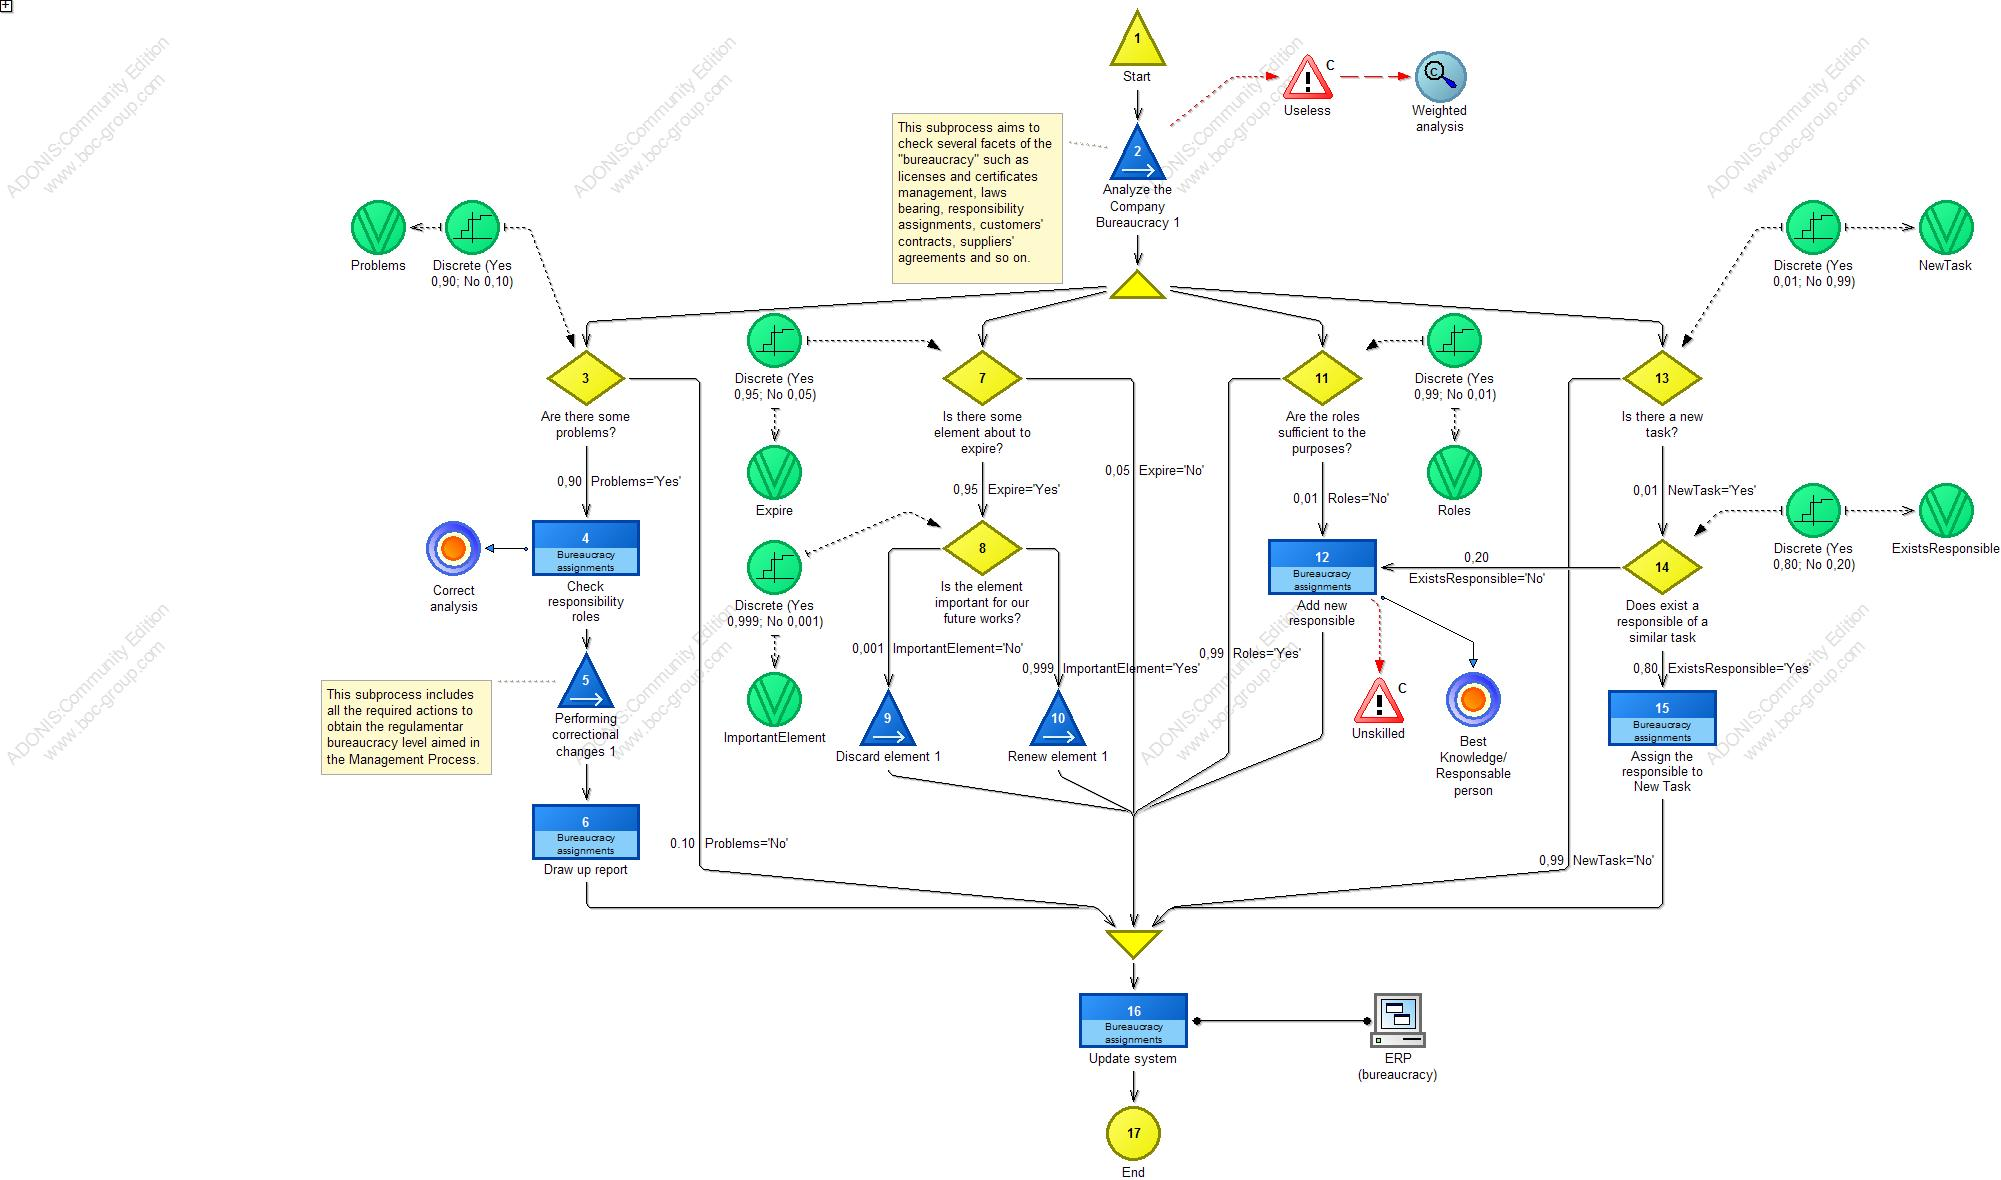
\includegraphics[scale=0.30]{assign2/adonis/imgs/financial_sup.jpg}
\caption{AllSpark financial support.}
\label{2img:financial_sup}
\end{centering}
\end{figure}


\subsubsection{Path Analysis}
The path analysis shows fifteen paths which three of them really important. The following table illustrate their characteristics.

\begin{table}[ht!]
\centering
\begin{tabular}{|l|l|l|l|l|}
\hline
Path&Probability&Execution time&Cycle time&Costs\\
\hline
1&0,6120&00:000:02:15:00&00:000:03:01:00&66,20\\
\hline
2&0,1650&00:000:02:55:00&00:000:03:01:00&116,20\\
\hline
3&0,1010&00:000:03:05:00&00:000:03:16:00&66,20\\
\hline
\end{tabular}
\end{table}

The favorite path is the first, with the expected probability of 0,6120\% due to the decision of ``Does exist a responsible of a simila task?''. It would useful to improve this point structuring a stronger  and it is presented as follows.\\

\begin{alltt}
Probability:   61,2000\%
Execution time:  00:000:02:15:00
Waiting time:  00:000:00:28:00
Resting time:  00:000:00:18:00
Transport time:  00:000:00:10:00
Cycle time:  00:000:03:01:00
Costs:  66,200000

Financial support 0.2 (Business process model)
========================================
Process start: Start
Parallelity: Parallelity-37548
    *
    Activity: Loading financial data
    *
    Activity: Focusing the task
    Decision: Are the owned skills sufficients? --> OwnedKnowledge='Yes'

Merging: Merging-37551
Activity: Perform business activity
Activity: Update Company information
Parallelity: Parallelity-37615
    *
    Decision: Is the financial status of AllSpark right? --> FinancialStatusOk='Yes'
    *
    Decision: Company is working right? --> WorkingOk='Yes'
    Activity: Next trend
    *
    Decision: Is AllSpark ready for change? --> TimeChanging='No'
Merging: Merging-37618
Activity: Draw up report and notify results to CEO
End: End
\end{alltt}


\subsubsection{Capacity Analysis}
The capacity analysis of the process figures as expectations that the business consultant is the primary role in the task and basically the business process is a sequential step of his work. In the analysis there is a great difference between the Cycle time and the Execution time and this is due to the time spent by the Business Operator in its tasks. A solution may be a better parallelization of the critical activity in order to standardize the outputting time.

\begin{landscape}
\centering
\begin{table}
{\tiny
\begin{tabular}{|l|l|l|l|l|l|l|}
Business process&Activity&Performer&Number&Execution time&Cycle time&Costs\\
\hline
Financial support 0.2&&&&00:000:02:33:28&00:000:03:04:50&77,040900\\
\hline
&Loading financial data&&1,000000&00:000:00:07:00&&0,300000\\
\hline
&&Business consultant&1,000000&00:000:00:07:00&&0,300000\\
\hline
&Focusing the task&&1,034000&00:000:00:10:20&&0,051700\\
\hline
&&Analyst&1,034000&00:000:00:10:20&&0,051700\\
\hline
&Update Company information&&1,000000&00:000:00:03:00&&0,800000\\
\hline
&&Secretary&1,000000&00:000:00:03:00&&0,800000\\
\hline
&Draw up report and notify results to CEO&&1,000000&00:000:00:20:00&&0,050000\\
\hline
&&Business consultant&1,000000&00:000:00:20:00&&0,050000\\
\hline
&Gathering informations&&0,034000&00:000:00:01:01&&0,027200\\
\hline
&&Business consultant&0,034000&00:000:00:01:01&&0,027200\\
\hline
&Plan a suggetion strategy&&0,229000&00:000:00:09:10&&11,450000\\
\hline
&&Business consultant&0,229000&00:000:00:09:10&&11,450000\\
\hline
&Historical study&&0,022000&00:000:00:00:26&&0,022000\\
\hline
&&Secretary&0,022000&00:000:00:00:26&&0,022000\\
\hline
&Plan changing&&0,170000&00:000:00:08:30&&0,000000\\
\hline
&&Business consultant&0,170000&00:000:00:08:30&&0,000000\\
\hline
&Next trend&&0,978000&00:000:00:44:01&&29,340000\\
\hline
&&Business consultant&0,978000&00:000:00:44:01&&29,340000\\
\hline
&Perform business activity&&1,000000&00:000:00:50:00&&35,000000\\
\hline
&&Business consultant&1,000000&00:000:00:50:00&&35,000000\\
\hline
Total&&&&00:000:02:33:28&&77,040900
\end{tabular}
}
\caption{Capacity analysis for Financial support.}
\end{table}
\end{landscape}
%

%

\subsection{Marketing Management}
The Marketing Management business process has to promote the Company's product to the business. The campaign can be structured in several manners, with access to different media and having various targets. The primary scope of the process is to perform the best work using historical data and analyzing the results in order to improve future campaigns. Figure \ref{2img:mark_man} shows the process in its wide.

The interested performers are primary the business consultant and CEO who are supported by the secretary in the different facets of the job.

\begin{figure}[ht!]
\begin{centering}
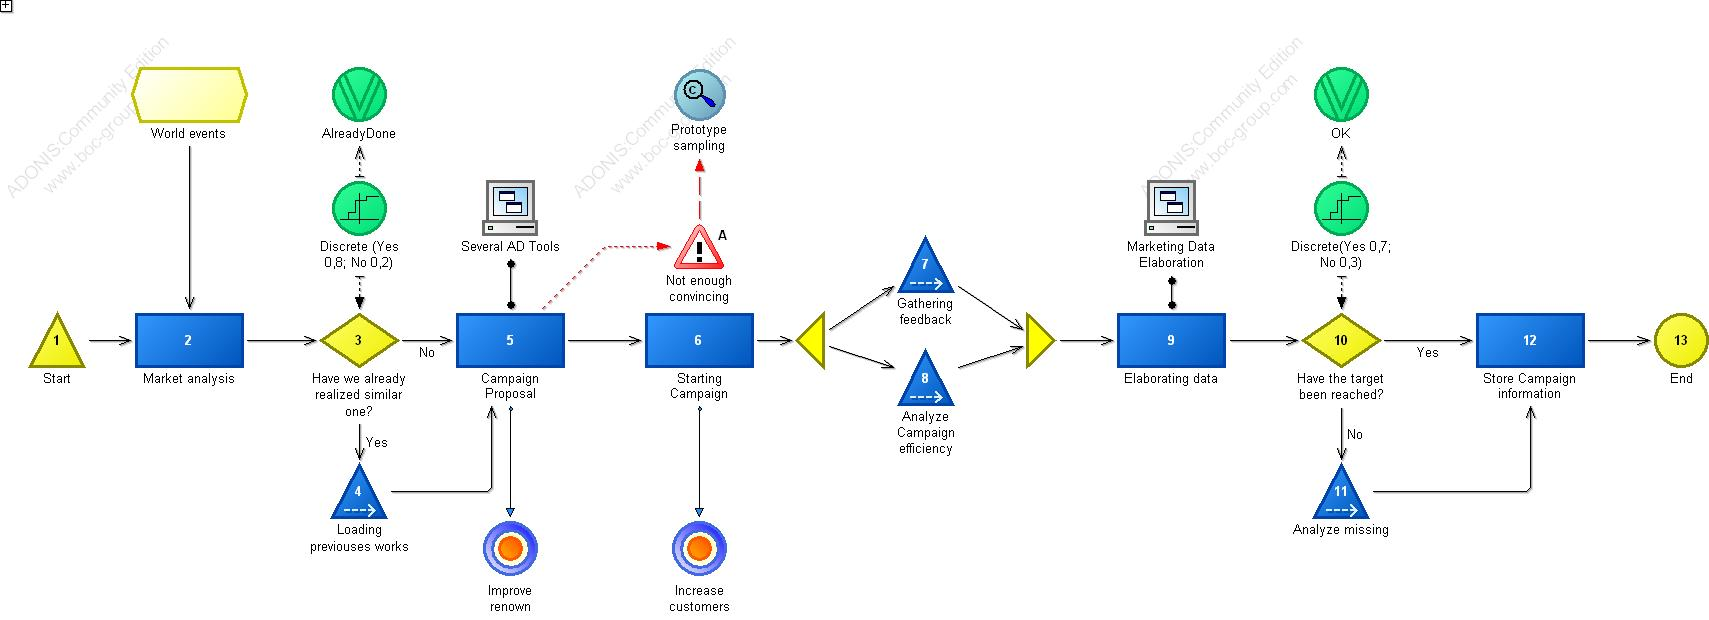
\includegraphics[scale=0.27, angle=90]{assign2/adonis/imgs/mark_man.jpg}
\caption{AllSpark Marketing Management.}
\label{2img:mark_man}
\end{centering}
\end{figure}


\subsubsection{Path Analysis}
The analysis of possible paths results the correspondence with interesting probability, one of them with the 56,70\% of probability to be performed. The analysis returns that paths have very similar time and costs and so are not so significative in the study of this process; this means that the Company has standardized the process to be more or less as expectations. The highest probability path is reported straight after the following table.

\begin{table}[ht!]
\centering
\begin{tabular}{|l|l|l|l|l|}
\hline
Path&Probability&Execution time&Cycle time&Costs\\
\hline
1&0,5670&00:018:07:50:00&00:001:00:25:00&2207,80\\
\hline
2&0,2140&00:018:08:35:00&00:001:00:25:00&2208,10\\
\hline
3&0,1450&00:018:07:40:00&00:001:00:25:00&2207,05\\
\hline
\end{tabular}
\end{table}

% \vspace

\begin{alltt}
Probability:   56,7000%
Execution time:  00:018:07:50:00
Waiting time:  00:001:00:25:00
Resting time:  00:001:00:23:00
Transport time:  00:000:03:28:00
Cycle time:  00:021:01:46:00
Costs:  2207,800000

Marketing Management 0.1 (Business process model)
========================================
Process start: Start
Activity: Market analysis
Decision: Have we already realized similar one? --> AlreadyDone = 'Yes'
Subprocess: Loading previouses works
Activity: Campaign Proposal
Activity: Starting Campaign
Parallelity: Parallelity-28827
    *
    Subprocess: Gathering feedback
    *
    Subprocess: Analyze Campaign efficiency
Merging: Merging-28833
Activity: Elaborating data
Decision: Have the target been reached? --> TargetReached = 'Yes'
Activity: Store Campaign information
End: End

Marketing Management 0.1 (Business process model) --> Loading previouses works 1 (Business process model)
========================================
Process start: Start
Activity: Loading Previouses works
End: End

Marketing Management 0.1 (Business process model) --> Gathering feedback 1 (Business process model)
========================================
Process start: Start
Activity: Gathering feedback
End: End

Marketing Management 0.1 (Business process model) --> Analyze campaign efficiency 1 (Business process model)
========================================
Process start: Start
Activity: Analyze campaign efficiency
End: End
\end{alltt}


\subsubsection{Capacity Analysis}
The capacity analysis of the process illustrates the specified timing and costs forseen for the single activities. Morevover it exlicities the Performer associated to each activity in order to check the responsibility for each step of the Business Process.

In this process the timing are very huge since the activities work on ``human'' domain and in particular the campaign commitment has to be completed before going to next activity. The difference between the Cycle time and Execution time is however curious since it is very wide. The motivation of this difference comes out from waiting and resting time elencated in the table above path analysis. This is a well known issue that arise in human to human reports and the only way to improve is to reduce the dead-time if the internal AllSpark's policy agree.

\begin{landscape}
\centering
\begin{table}
{\tiny
\begin{tabular}{|l|l|l|l|l|l|l|}
Business process&Activity&Performer&Number&Execution time&Cycle time&Costs\\
\hline
Marketing Management 0.1&&&&00:018:08:00:59&00:021:01:56:46&2207,876650\\
\hline
&Market analysis &&1,000000&00:001:08:20:00&&200,000000\\
\hline
&&Business consultant &1,000000&00:001:08:20:00&&200,000000\\
\hline
&Campaign Proposal &&1,000000&00:000:08:00:00&&1000,000000\\
\hline
&&CEO &1,000000&00:000:08:00:00&&1000,000000\\
\hline
&Starting Campaign &&1,000000&00:015:00:00:00&&1000,000000\\
\hline
&&CEO &1,000000&00:015:00:00:00&&1000,000000\\
\hline
&Elaborating data &&1,000000&00:001:00:00:00&&7,000000\\
\hline
&&Secretary &1,000000&00:001:00:00:00&&7,000000\\
\hline
&Store Campaign information &&1,000000&00:000:00:30:00&&0,400000\\
\hline
&&Secretary &1,000000&00:000:00:30:00&&0,400000\\
\hline
&Loading Previouses works &&0,793000&00:000:00:07:56&&0,039650\\
\hline
&&Secretary &0,793000&00:000:00:07:56&&0,039650\\
\hline
&Gathering feedback &&1,000000&00:000:00:20:00&&0,050000\\
\hline
&&Area Manager &1,000000&00:000:00:20:00&&0,050000\\
\hline
&Analyze campaign efficiency &&1,000000&00:000:00:30:00&&0,300000\\
\hline
&&Area Manager &1,000000&00:000:00:30:00&&0,300000\\
\hline
&Analyze missing &&0,290000&00:000:00:13:03&&0,087000\\
\hline
&&Area Manager &0,290000&00:000:00:13:03&&0,087000\\
\hline
Total&&&&00:018:08:00:59&&2207,876650\\
\end{tabular}
}
\caption{Capacity analysis for Marketing management.}
\end{table}
\end{landscape}
%

%

\subsection{Public Relation Management}
The Public Relation Management aims to standardize the way how Company undertakes relations with customers, or future ones, in order to improve its  basket of possible purchasers. Basically the Manager assigned to supervise the Company's public face organize the way, the method and the information that the Representative, or the Analyst in some rare case\footnote{The analyst is not responsible to public relation, but he can be required in the project's advanced stage to fit at best the customers' demands.}, who contacts direct the cutomer, is charged to divulgate. 

The Representative has to relates with the customer in a pleasant way in order to facilitate future relationships. Image \ref{2img:mark_man} represent the process modeled.

During the process may be requested the support of the Secretary and the authorizations of the CEO. Also important is the Business operator who should regulate the different necessity of the Representative.

\begin{figure}[ht!]
\begin{centering}
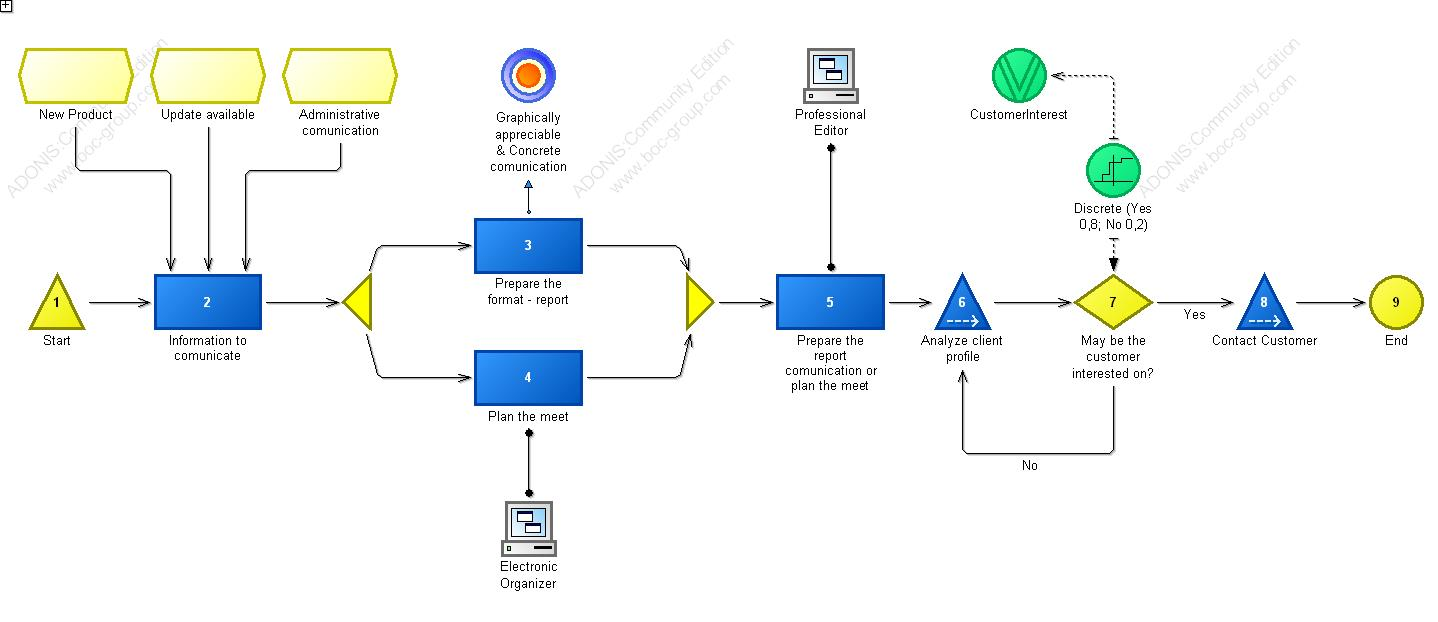
\includegraphics[scale=0.33, angle=90]{assign2/adonis/imgs/pr_man.jpg}
\caption{AllSpark Public Relation Management.}
\label{2img:pr_man}
\end{centering}
\end{figure}


\subsubsection{Path Analysis}
The Public Relation Management path analysis results the expected value of a high probability in contacting the customer, that is 80,40\%. The following table illustrate a huge amount of time, expecially the waiting time, but is important to evidence that is a process strongly linked to human timing such as movement in the physical world, report compilation and meetings.

The forseen costs indicate mainly the transfer expenses which are for the majority charged to the Company.

Interesting is that the relation management may happen also in through Internet and so both costs and time are very huge, but is difficult to relate with another person through the Network unless explicity required. The main objective of the Company is to reach directly the customer in the nearest places, but connecting with mail, videoconference and telephone the farest ones who may require direct high level personnel for specified tasks.

\begin{alltt}
Probability:   81,4000%
Execution time:  00:000:03:00:00
Waiting time:  00:000:00:51:00
Resting time:  00:000:00:14:00
Transport time:  00:000:00:30:00
Cycle time:  00:000:04:22:00
Costs:  33,800000

Public Relation Management 0.1 (Business process model)
========================================
Process start: Start
Activity: Information to comunicate
Parallelity: Parallelity-29253
    *
    Activity: Prepare the format - report
    *
    Activity: Plan the meet
Merging: Merging-29256
Activity: Build or group elements to comunicate
Subprocess: Analyze client profile
Decision: May be the customer interested on? --> CustomerInterest = 'Yes'
Subprocess: Contact Customer
End: End

Public Relation Management 0.1 (Business process model) --> Analyze client profile 1 (Business process model)
========================================
Process start: Start
Activity: Analyze client profile
End: End

Public Relation Management 0.1 (Business process model) --> Contact customer 1 (Business process model)
========================================
Process start: Start
Activity: Contact customer
End: End
\end{alltt}


\subsubsection{Capacity Analysis}
The capacity analysis shows the time simulated with the model and the importance of that is give by the activies of which are very time spending. Apart the ``Contact customer'', the others may be overcharged since the execution time is really high. The explanation is that the center of the realation is another person and so a good comunication make easier each future relationship and so the high time is motivated by a research on the best way to relate with a third party.

\begin{landscape}
\centering
\begin{table}
{\tiny
\begin{tabular}{|l|l|l|l|l|l|l|}
Business process&Activity&Performer&Number&Execution time&Cycle time&Costs\\
\hline
Public Relation Management 0.1&&&&00:000:03:07:12&00:000:04:30:24&33,848000\\
\hline
&Information to comunicate &&1,000000&00:000:00:30:00&&0,200000\\
\hline
&&Area Manager &1,000000&00:000:00:30:00&&0,200000\\
\hline
&Build or group elements to comunicate &&1,000000&00:000:00:20:00&&0,200000\\
\hline
&&Representative &1,000000&00:000:00:20:00&&0,200000\\
\hline
&Prepare the format - report &&1,000000&00:000:00:40:00&&3,000000\\
\hline
&&Representative &1,000000&00:000:00:40:00&&3,000000\\
\hline
&Plan the meet &&1,000000&00:000:00:10:00&&0,200000\\
\hline
&&Representative &1,000000&00:000:00:10:00&&0,200000\\
\hline
&Contact customer &&1,000000&00:000:00:50:00&&30,000000\\
\hline
&&Representative &1,000000&00:000:00:50:00&&30,000000\\
\hline
&Analyze client profile &&1,240000&00:000:00:37:12&&0,248000\\
\hline
&&Area Manager &1,240000&00:000:00:37:12&&0,248000\\
\hline
Total&&&&00:000:03:07:12&&33,848000\\
\end{tabular}
}
\caption{Capacity analysis for Public Relation Management.}
\end{table}
\end{landscape}
%

%